% p1)	reintroduces problem, and what decisions we had to make
% 			- which features
% 			- which classifier SVM vs NB
% 			
% p2) Part-of-speech tagging
% 
% p3)	Subj clues
% 
% p3)	Other features
% 
% p4) Choosing features
% 
% p5) Choosing NB or SVM
% 
% p6) Results
% 
% p7) Evaluation

% Give example tweet and calculate feature set for it, then give output classification.
% 
% EngTagger changes:
% 	- often names are lower case e.g. joseph -> Joseph
% 	- added handling for @mentions
% 
% If using a lexicon, look at it's coverage over the training set, i.e. does each subjective word in the lexicon exist in one or more examples. How many subjective examples do not contain words from the subjective lexicon?

\chapter{Subjectivity classification}
\label{subjectivity}

Once a status has been retrieved, the first step towards understanding it's sentiment lies in determining whether it is subjective or objective. This is known as subjectivity classification and it serves as the first stage within our sentiment analysis engine. In classifying subjectivity we decided to take a supervised approach to the problem. This is largely due to the fact, that as Wiebe and Riloff observe \cite{Wiebe:2003wa}, although unsupervised approaches' precision rates are high, achieving high recall rates is remarkably difficult. As a result, the problem now lies in designing the elements which will best enable our supervised classifier to separate statuses into their correct labels.

In this chapter we shall first examine how we built our training set, and the decisions behind our labelling. With a training set in place, we will then go on to explore the features we think will be of value, along with the reasoning behind them and a discussion of their implementation. We shall then go on to look at the results of our tests, examining which feature combinations performed best and why, along with which classification method best suited the problem. Finally we shall evaluate our classifiers performance against the results commonly seen in literature.

\section{Training set}
\label{subjectvity:training}

Before we can build a classifier, we need to assemble a training set which best represents the domain of our problem. Furthermore in assembling our training set, we also want to be able to annotate it so as to better explain our decisions. Although we have already discussed our approach to labelling data in chapter \ref{retrieval}, we shall examine what aspects of our approach particularly relate to subjectivity classification within the remainder of this section.

Our approach to subjectivity classification takes a two label approach of either \emph{subjective} or \emph{objective}. Thus the first annotation we want to make to our \emph{TrainedStatus} class is one denoting subjectivity. Accordingly each \emph{TrainedStatus} is given an \texttt{subjective} attribute, which takes a value of either "\emph{t}" or "\emph{f}". Alongside this we want to collect a more detailed picture of why exactly the status is subjective. In order to do this we collect the phrases which have implied subjectivity in a \texttt{phrases} array. Although for the purposes of polarity classification we will eventually have to divide our \texttt{phrases} array into two, for now all we are interested in is collecting subjective phrases, but not annotating them with any additional sentiment detail.

With each status now annotated with its subjectivity label and an array of any subjective phrases, we can focus on building our feature set and training our classifier.

\section{Features}

As with any classification problem, picking a suitable feature set is decisive in classification performance. In implementing our classifier we chose to draw upon a range of previously successful features, along with our own new or adapted ones. In this section we shall examine why and how we implemented our chosen features, but will save a discussion of their effectiveness and final selection until later in this chapters's results and evaluation sections.

\subsection{Adjectives}

As discussed in the background section, adjectives are often regarded as strong indicators of subjectivity. With our status' POS tags readily available through its \texttt{parts\_of\_speech} method, we now need to extract those words which our used as adjectives. Within our tagset however, there are four different tags representing adjectives. In order to handle this, we added a \texttt{general(pos)} method to our \emph{TweetTagger} class. This method takes a specific tag, such as "\emph{jjr}" or "\emph{adr}", and returns its more general tag, in this case "\emph{adj}" or "\emph{adverb}". This is done by comparing the specific tag against regular expressions corresponding to the general tags. These general tags, their meaning and their regular expression can be seen in table \ref{table:regex_pos}.

With a method now available for identifying tags as adjectives, we can focus on how we collect those adjectives for any given status. As this a method corresponding to an attribute of our status, i.e. its adjectives, we decided to implement this as an \texttt{adjectives} method within our \emph{Status} class, as included in listing \ref{classifiers:status_adjectives}.

\begin{lstlisting}[language=Ruby, caption={\emph{Status} object's \texttt{adjective} method for returning all parts of speech used as adjectives}, label=classifiers:status_adjectives]
def adjectives
  self.parts_of_speech.select{|pos| TweetTagger.general(pos["tag"]) == "adj"}
end
\end{lstlisting}

It is important to note that the design decision to keep methods such as adjective collection within the \emph{Status} object is consistent throughout our implementation. With a status' adjectives now easily accessible we were able to build our two adjective-based feature methods:

\begin{description}
	\item [\texttt{has\_adjectives?}] returns a boolean value denoting adjective presence within the status.
	\item [\texttt{no\_adjectives}] returns one of three values based upon the number of adjectives. For zero adjectives, \texttt{0} is returned, for one or two adjectives, \texttt{1} is returned and for three or more adjectives \texttt{2} is returned.
\end{description}

\subsection{URLs}

Our approach to URLs was implemented in a similar to that taken for adjectives. We first implemented a \texttt{urls} method for all \emph{Status} objects, implementing it in a similar fashion to the \texttt{adjectives} method. Using this, we were then able to build our two url-based feature methods:

\begin{description}
	\item [\texttt{has\_urls?}] returns a boolean value denoting URL presence within the status.
	\item [\texttt{no\_urls}] returns one of three values based upon the number of URLs. For zero URLs, \texttt{0} is returned, for one or two URLs, \texttt{1} is returned and for three or more URLs \texttt{2} is returned.
\end{description}

\subsection{Mentions}

\subsection{Subjective clues}

As originally observed by Wiebe and Riloff \cite{Wiebe:2000ub}, subjective clues often prove to be effective discriminators when classifying subjectivity. In effect, this is done by compiling a list of clue words, alongside their subjectivity strength, in our case \emph{weak} or \emph{strong}. Furthermore the word's part of speech tag is noted, so as to ensure that the word being marked as a clue is in fact being used in the correct sense.

Our approach to clue finding uses the same lexicon as Wiebe and Riloff \cite{Wiebe:2000ub}. Alongside this we use out own lexicon of subjective phrases, by collecting our phrase annotations as described in section \ref{subjectvity:training}. The resultant clue lexicons are stored in regular text files, with each line consisting of one clue, as demonstrated in listing \ref{subjectivity:clues}.

\begin{lstlisting}[numbers=none, caption={Example clue from the subjective clue lexicon}, label=subjectivity:clues]
type=weaksubj len=1 word1=block pos1=noun stemmed1=n priorpolarity=negative
type=weaksubj len=1 word1=block pos1=verb stemmed1=y priorpolarity=negative
\end{lstlisting}

The \texttt{type} field represents whether a clue is \emph{strong} or \emph{weak}, while the \texttt{len} field denotes the length of the clue. The \texttt{word}, \texttt{pos} and \texttt{stemmed} fields represent the properties of each word in the clue's phrase, with \texttt{stemmed} indicating whether the clue applies to all un-stemmed versions of the word. For example, this means that not only is "\emph{block}" a clue in the above example, but so is the word "\emph{blocks}" when it is used as a verb. This is due to "\emph{block}" being the stem of "\emph{blocks}". Finally the \emph{priorpolarity} field denotes the polarity of the clue.

In order to find our clues, we implemented a singleton \emph{ClueFinder} class. The class loads each clue into a \texttt{clues} hashmap, in which each \emph{key} is a clue phrase, and it's \emph{value} is an array of all possible ways in which the phrase may be used as a subjective clue. An example item from the resultant hash is demonstrated in listing \ref{subjectivity:clues_hash}.

\begin{lstlisting}[language=Ruby, caption={Ruby hashmap representation of listing \ref{subjectivity:clues}}, label=subjectivity:clues_hash]
clues["block"]
	=> {[
		{:type => "weaksubj", :len => 1, :pos => ["noun"], :stemmed => ["n"], :priorpolarity => "negative"},
		{:type => "weaksubj", :len => 1, :pos => ["verb"], :stemmed => ["y"], :priorpolarity => "negative"}
	]}
\end{lstlisting}

With our clues now loaded in a hashmap, we defined a \texttt{clue\-\_data(words, pos)} method, which when given a phrase and array of words along with their corresponding POS tags, will check the hashmap to see if the combination does in fact represent a clue. If they do, the method will return the clue \texttt{type} and \texttt{priorpolarity}, otherwise it will simply return \texttt{nil}. Using this we can now easily define three useful methods for our \emph{Status} class, \texttt{subjective\-\_clues}, \texttt{weak\-\_subjective\-\_clues}, \texttt{strong\-\_subjective\-\_clues}. These methods simply iterate over the statuses unigrams, bigrams and trigrams each time checking to see if they represent a clue, before filtering them accordingly if we are looking for weak or strong clues.

With status methods now in place for easily retrieving clues, we can go on to build our six clue-based feature methods.

\begin{description}
	\item [\texttt{has\_subjective\_clues?}] returns a boolean value denoting the presence of one or more subjective clues
	\item [\texttt{no\_subjective\_clues}] returns one of three values based upon the number of subjective clues. For zero clues, \texttt{0} is returned, for one or two clues, \texttt{1} is returned and for three or more clues \texttt{2} is returned.
	\item [\texttt{has\_weak\_subjective\_clues?}] as with \texttt{has\-\_subjective\-\_clues?}, but only noting weak clues.
	\item [\texttt{has\_strong\_subjective\_clues?}] as with \texttt{no\-\_subjective\-\_clues}, but only noting strong clues.
	\item [\texttt{no\_weak\_subjective\_clues}] as with \texttt{has\-\_subjective\-\_clues?}, but only noting weak clues.
	\item [\texttt{no\_strong\_subjective\_clues}] as with \texttt{no\-\_subjective\-\_clues}, but only noting strong clues.
\end{description}

\subsection{Capitalised words}

As observed by Barbosa and Fang \cite{Barbosa:ws}, objective statuses tend to contain significant capitalisation. This is often a result of the status either being spam, or as increasingly the case, it is due to the status containing the HTML page title of the URL it is linking to. Accordingly, we experimented with two features based upon this:

\begin{description}
	\item [\texttt{capitalised\_word\_frequency}] {looks at the ratio of capitalised words to total word, i.e.
	\begin{equation}
		c.w.f = \frac{|words_{capitalised}|}{|words|}
	\end{equation}
	Rather than returning the floating point number, one of three values are returned. For all values between 0 and 0.3, we return \texttt{0}, for values between 0.3 and 0.5, we return \texttt{1} and for values greater than 0.5, we return \texttt{2}.
	}
	\item [\texttt{capital\_letter\_frequency}] looks at the ratio of capitalised letters to total letters, i.e.
	\begin{equation}
		c.l.f = \frac{|letters_{capitalised}|}{|letters|}
	\end{equation}
	Rather than returning the floating point number, one of three values are returned. For all values between 0 and 0.2, we return \texttt{0}, for values between 0.2 and 0.5, we return \texttt{1} and for values greater than 0.5, we return \texttt{2}.
\end{description}

\section{Results}

In this section we present our subjectivity classifier's performance across a variety of tests. In doing so we will observe how individual features and combinations of them perform, along with exploring the effect of different classifier types on overall performance. All tests are performed using three-fold cross validation over a set of 300 labelled tweets, and repeated 30 times to ensure an accurate measure.

\subsection{Individual feature performance}

In deciding a suitable feature set for our classifier, we first wanted to observe which features perform best on their own. In order to do this each individual feature was used to initialise our classifer, before running our test methods on each single-feature classifier. In order to truly understand the performance of each feature, we decided to focus on their \emph{accuracy}, \emph{precision} and \emph{recall}. For each measure we wanted to look at not only the average, but the spread of results across the 100 repetitions. This was so as to provide a better understanding as to the sensitivity of each measure to changes in its training data. We have presented our results for each measure below, and we shall now examine the results for each measure in turn.

It is important to note that in order to present our data in a tidier fashion, we will use the following numbering system when discussing and presenting features:

\begin{longtable}{|p{0.25in}|p{1.05in}|p{0.25in}|p{1.05in}|p{0.25in}|p{1.05in}|}
		\hline
		No. & Feature & No. & Feature & No. & Feature \\
		\hline
		1 & has\-\_adjectives? & 7 & has\-\_clues? & 13 & \multirow{3}{3pt}{capitalised\-\_words\-\_frequency} \\
		\cline{1-4}
    2 & no\-\_adjectives & 8 & no\-\_clues & & \\
		\cline{1-4}
    3 & has\-\_urls? & 9 & has\-\_strong\-\_clues? & & \\
		\hline
    4 & no\-\_urls & 10 & no\-\_strong\-\_clues & 14 & \multirow{3}{3pt}{capitalised\-\_letters\-\_frequency} \\
		\cline{1-4}
    5 & has\-\_mentions? & 11 & has\-\_weak\-\_clues? & & \\
		\cline{1-4}
		6 & no\-\_mentions & 12 & no\-\_weak\-\_clues & & \\
		\hline
\end{longtable}

In figures \ref{fig:subj_a}, \ref{fig:subj_p} and \ref{fig:subj_r} we present the test results for each of our single-feature classifiers.

\begin{figure}
	\caption{Accuracy average and spread for each individual feature}
	\label{fig:subj_a}
	\centering
		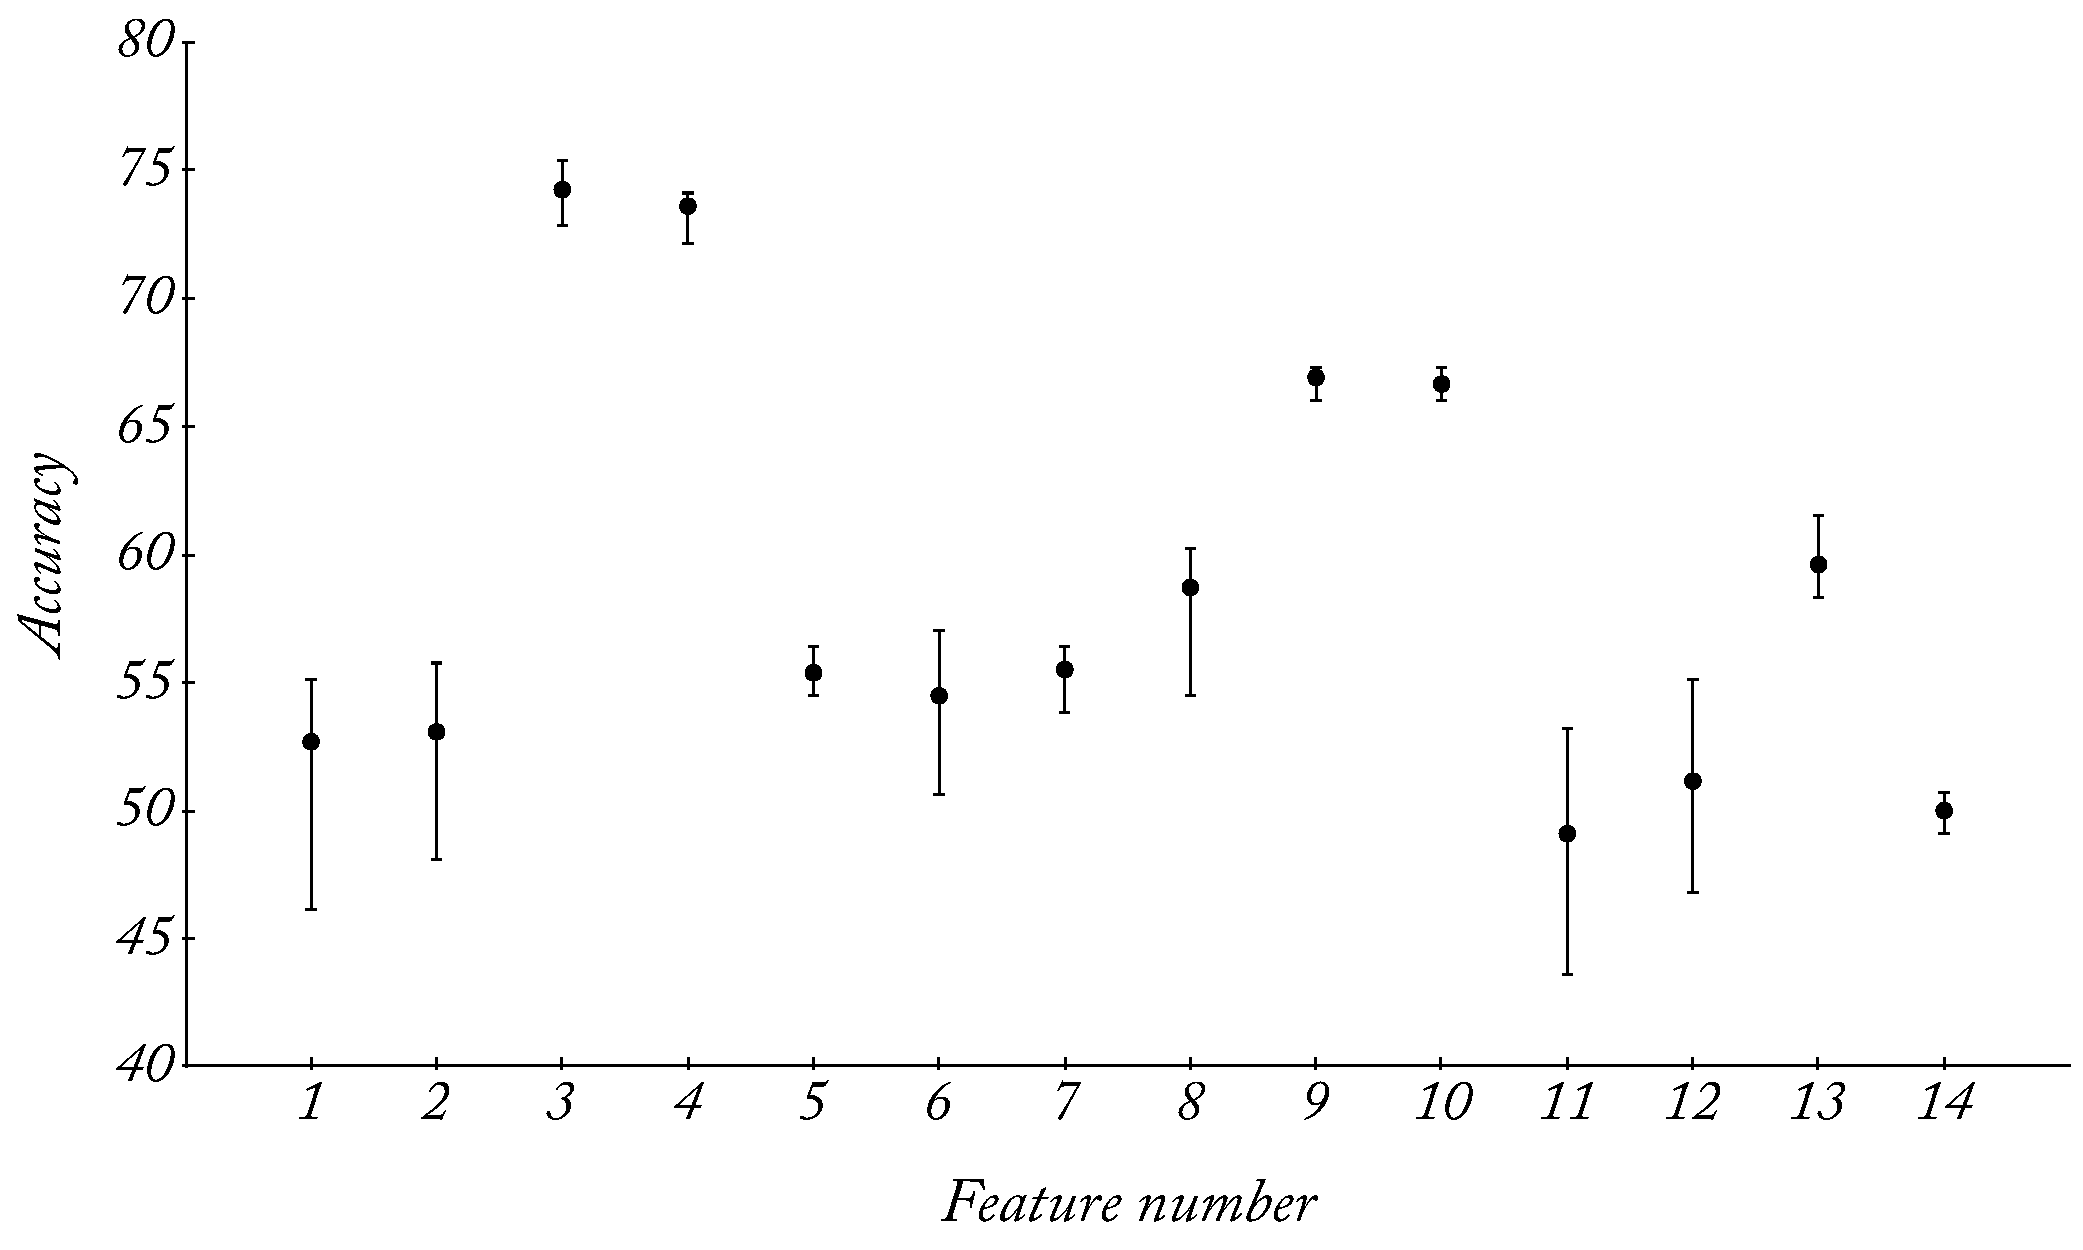
\includegraphics[width=1.0\textwidth]{graphs/subj_a.pdf}
\end{figure}

We found that URLs and strong subjectives clues were the most informative feature in terms of accuracy. URLs are clearly the most discriminative feature, and when used as a presence-based feature heralded an average classification accuracy of 72.84\%. The presence of strong subjective clues also served as a particularly discriminative feature, classifying 66.9\% of examples correctly when used as a presence-based feature. Furthermore, when used as individual features, we found that URLs and strong subjective clues presented little spread in our accuracy results. This suggests that unlike features such as adjectives or weak subjective clues, URLs and strong subjective clues are not sensitive to changes in training data. Interestingly however, we also found that there was little change in accuracy when basing a feature on presence or number of occurrences within the status. All our features, other than weak subjective clue presence, resulted in accuracies greater than 50\%. As such, although some do little better than simply guessing, most offer at least some additional insight when classifying a status' subjectivity.

\begin{figure}
	\caption{Precision average and spread for each individual feature}
	\label{fig:subj_p}
	\centering
		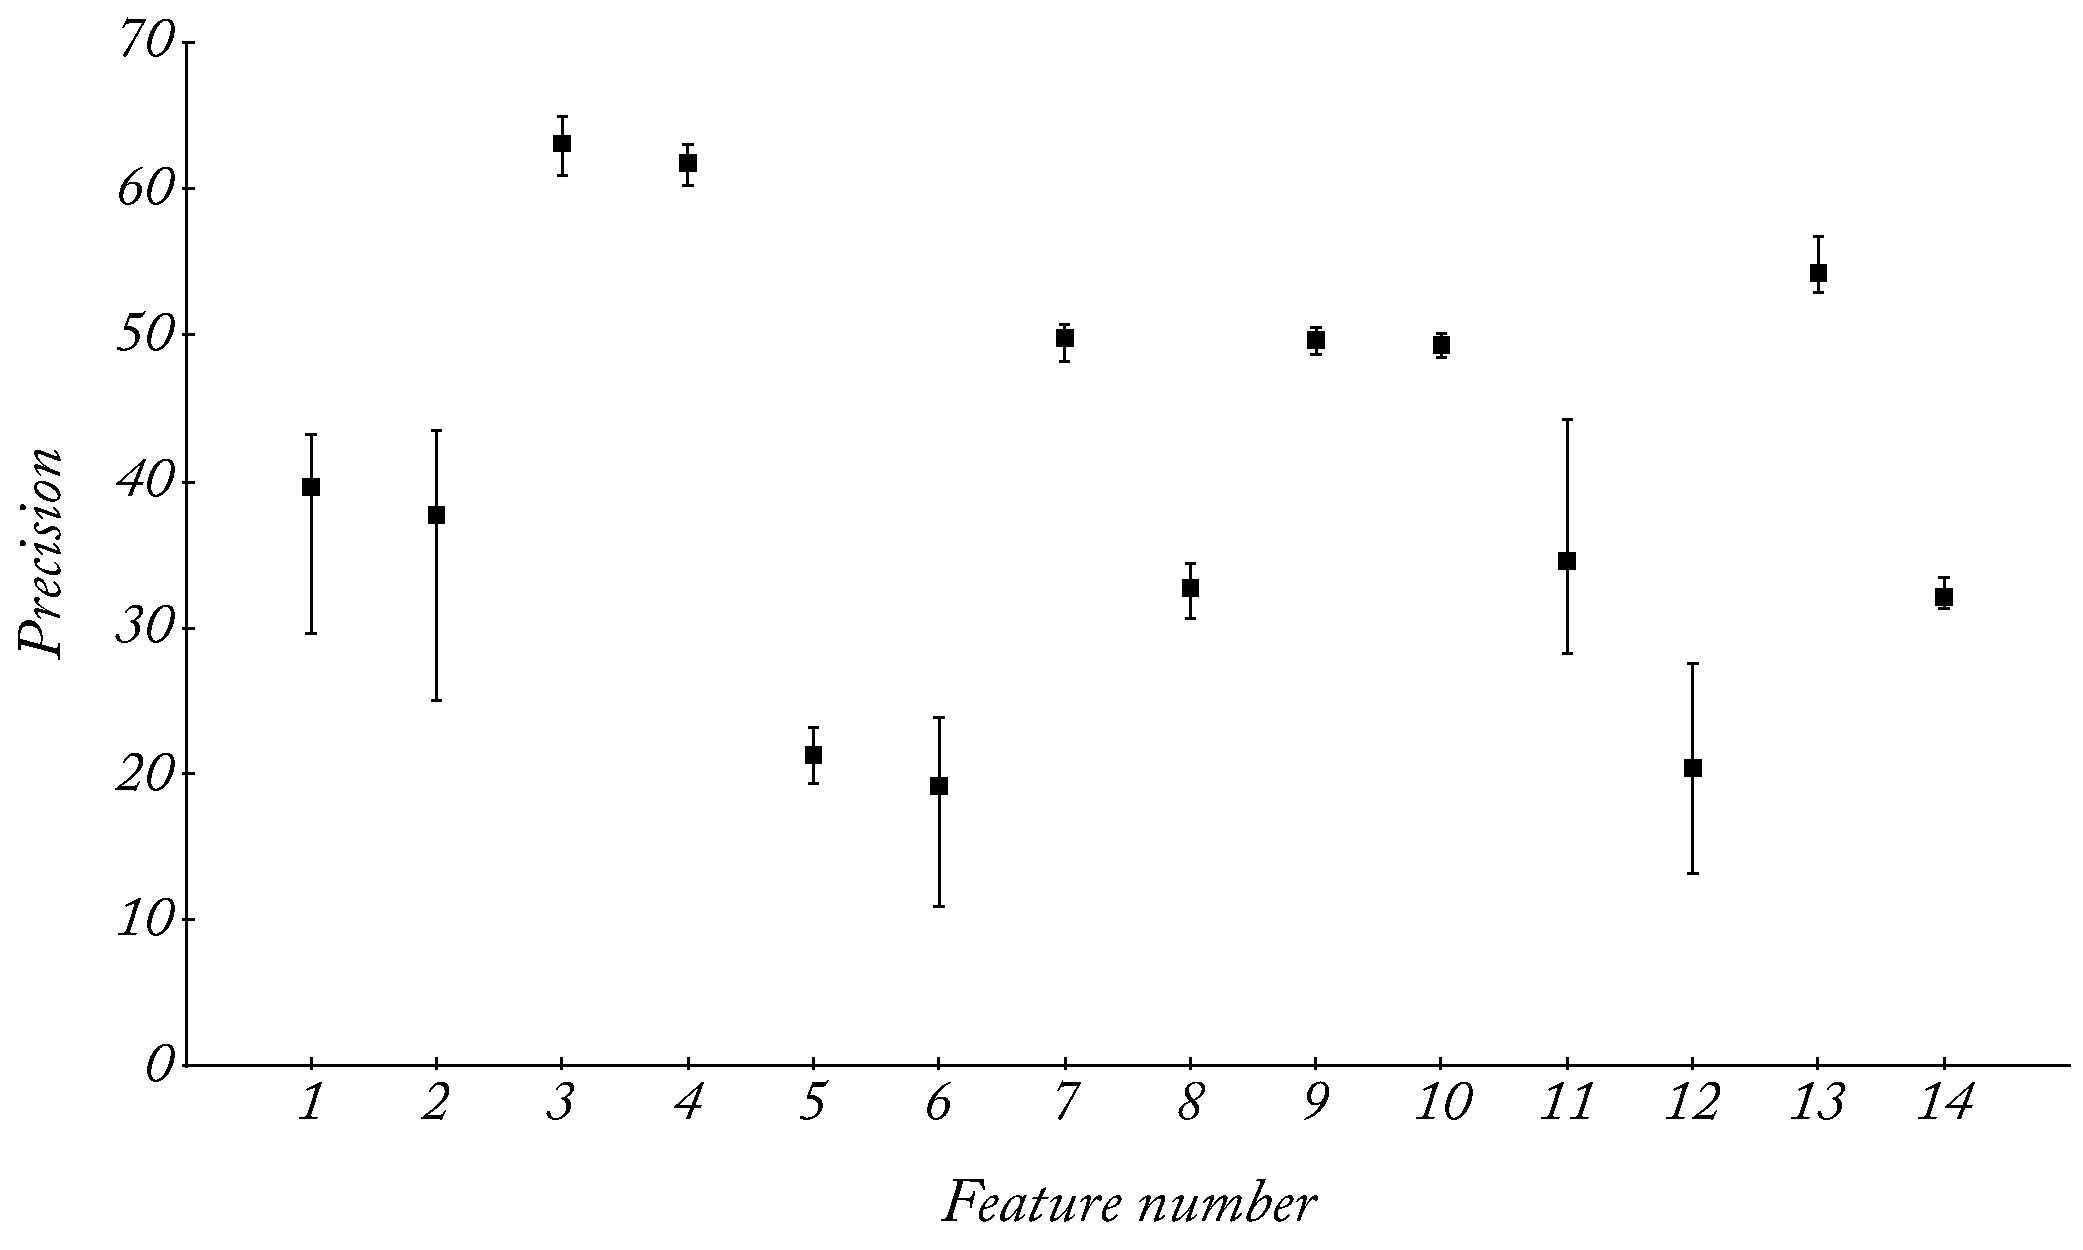
\includegraphics[width=1.0\textwidth]{graphs/subj_p.pdf}
\end{figure}

In general, we found that features on their own presented little in the way of precision. As with accuracy, URLs again offered the best as far as precision rates were concerned, with precision rates of 63.1\% when used as a presence-feature and 61.8\% when the number of occurrences was taken into account. Also of note was our capitalised words feature which achieved a precision rate of 54.3\%. Again weak subjectives performed weakly as a feature, and both it and adjectives suggested that their sensitivity to changes in training data made them unreliable.

\begin{figure}
	\caption{Recall average and spread for each individual feature}
	\label{fig:subj_r}
	\centering
		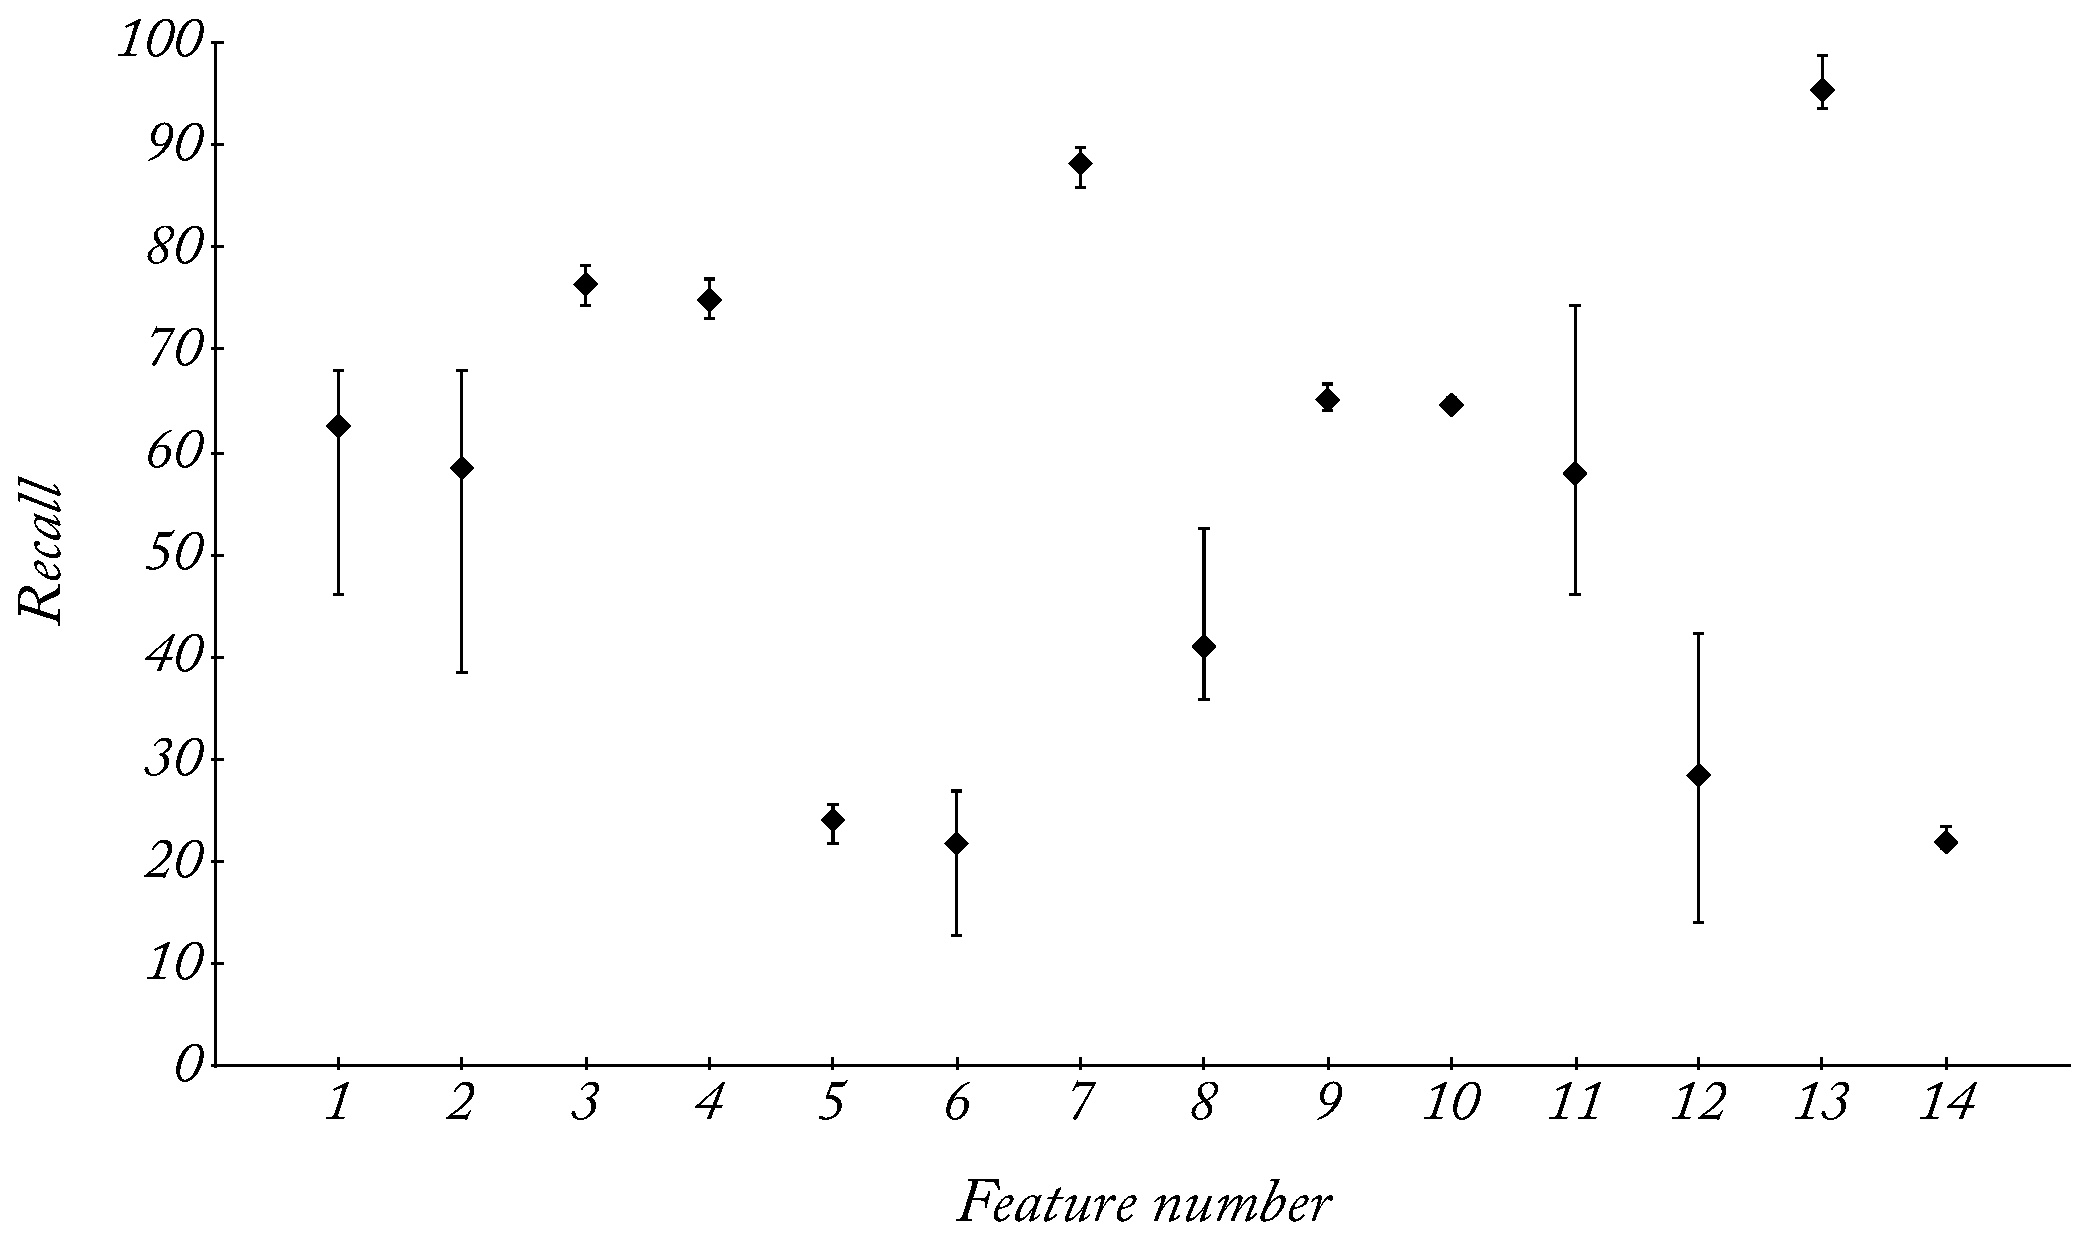
\includegraphics[width=1.0\textwidth]{graphs/subj_r.pdf}
\end{figure}

Recall rates proved much better for our features. This is probably largely due to the one sided-ness of much of their classification, especially in the case of capitalised words, which labelled almost 100\% of its test data as subjective. Of note however are the high recall rates achieved by URLs and strong subjective clues, which we had already identified as strong potential features. Again adjectives and weak subjective clues demonstrated their tendency to be strongly affected by changes in training data, suggesting their potential unsuitability for subjectivity classification. For adjectives, this is strongly at odds with prior research in the field, and as a result we will further experiment with it when testing how our classifier performs with groups of features.

\subsection{Feature set performance}
\label{subjectivity:feature_set}

As a result of our individual feature analysis, we put forward five feature-combinations for further testing:

\begin{enumerate}
	\item has\_urls?, has\_strong\_clues?
	\item has\_urls?, has\_strong\_clues?, no\_clues
	\item has\_urls?, has\_strong\_clues?, capitalised\_words\_frequency
	\item has\_urls?, has\_strong\_clues?, no\_clues, capitalised\_words\_frequency
	\item has\_urls?, has\_strong\_clues?, no\_clues, capitalised\_words\_frequency, has\_adjectives?
\end{enumerate}

The results of our tests using the five feature sets are listed in figure \ref{fig:subj_multi}. Blue bars represent precision, red represents accuracy and green represents recall.

\begin{figure}
	\caption{Precision (square), accuracy (circle) and recall (diamond) results for our five different feature sets.}
	\label{fig:subj_multi}
	\centering
		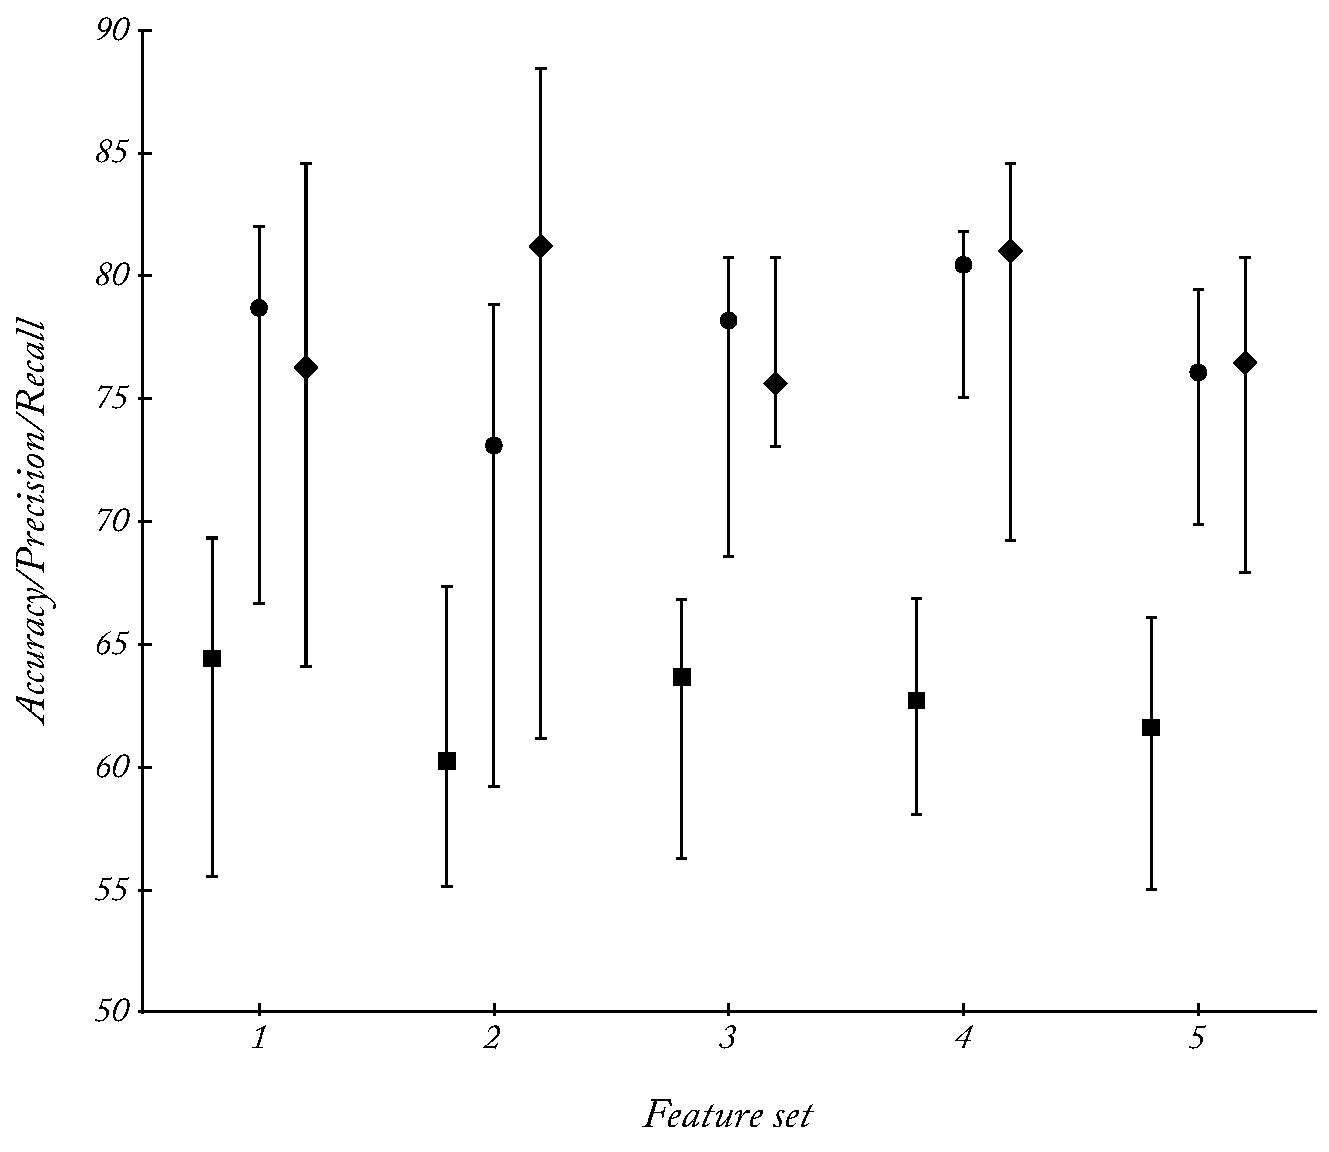
\includegraphics[width=0.9\textwidth]{graphs/subj_multi.pdf}
\end{figure}

All classifiers perform well, with our fourth feature set performing strongest in terms of accuracy achieving an average of 80.5\%. It performed marginally worse that feature set two with regards to precision, scoring an average of 81.0\%. Although it's precision was not the best, its strong accuracy and recall, combined with it's low sensitivity to changes in the training set, make it our preferred feature set. Interestingly adjectives seemed to have an adverse effect on our overall accuracy, precision and recall.

\subsection{Classifier type}

In order to determine the most appropriate classifier type, we ran our tests using a Support Vector Machine for one test and a Naive Bayes Classifier for the other. When building our classifiers, we used the fourth feature set from section \ref{subjectivity:feature_set}. We present our results in figure \ref{fig:subj_class}.

\begin{figure}
	\caption{Precision (square), accuracy (circle) and recall (diamond) results for SVM and NB classifier.}
	\label{fig:subj_class}
	\centering
		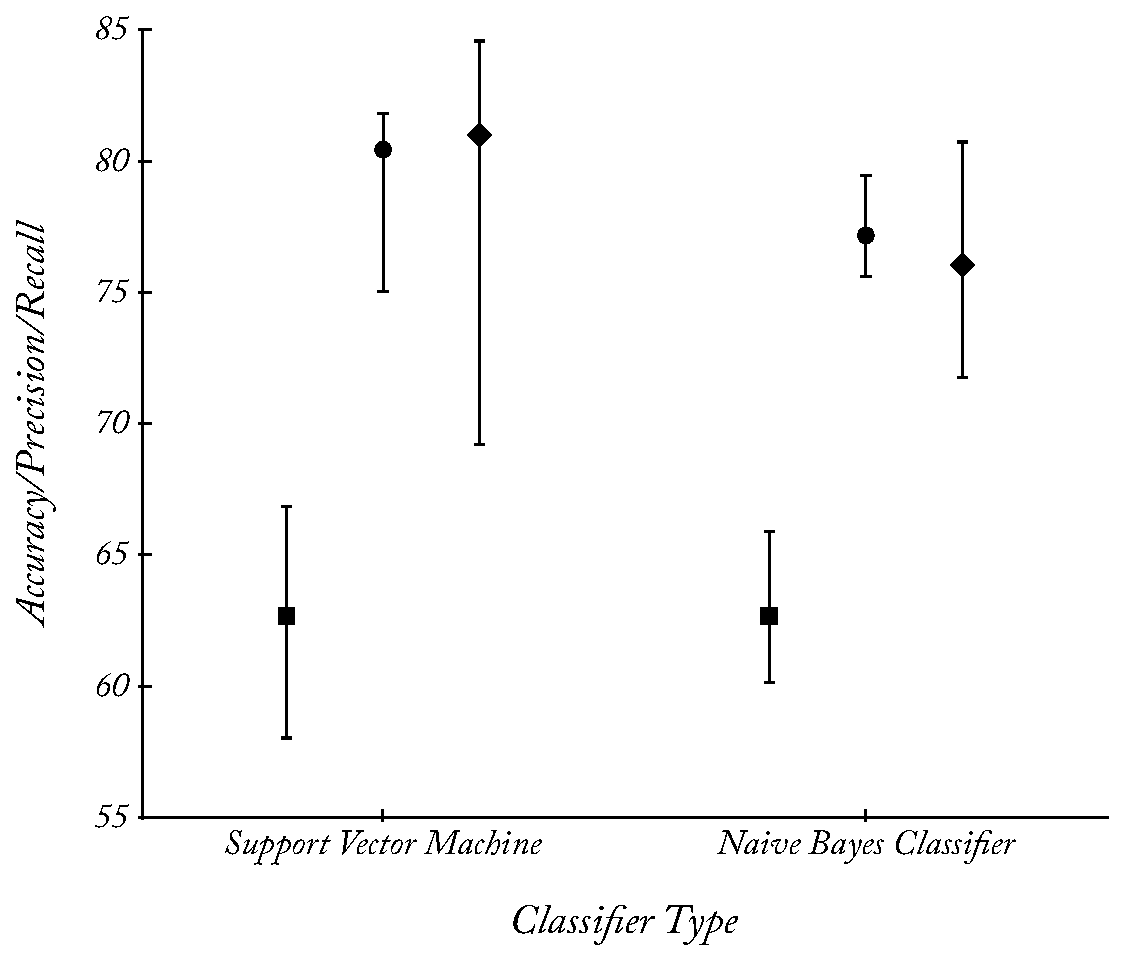
\includegraphics[width=0.8\textwidth]{graphs/subj_class.pdf}
\end{figure}

In terms overall performance, there is little difference between our SVM and NB performance. Overall SVM slightly outperforms NB in terms of accuracy with an average of 72.7\% against the NB average of 71\%. We feel however that in the future if the amount of training data we have is to increase, the SVM would provide a more robust and useful classification method.

\section{Evaluation}

Our subjectivity classification rates were strong. With an average accuracy of 80.5\%, our classifiers performance further improved upon results typically seen in the field, such as the average accuracy of 70.2\% seen by Wiebe et al. \cite{Wiebe:2000tk}. The class itself was both simple to use, and train, though this was largely due to the success of our \emph{Classifier} class implementation. We used a good blend of both linguistic features and Twitter meta-features such as URLs, and as a result saw strong classification rates.

In future work there are five areas in particular which we would look to for further improvement,

\begin{description}
	\item [Training set size] - Overall we felt that the limited size of our training set limited our classifiers ability. In future work we would spend more time building up a much more significant amount of labelled data.
	\item [Word-sense disambiguation] - Although we use part-of-speech tagging to distinguish between the grammatical usage of words, word-sense disambiguation may have seen a further improvement in results. In distinguishing between the senses of words, we provide ourselves with a more dtailed account of their use and are thus better informed when classifying subjectivity.
	\item [No URL feature] - The presence of URLs proved to be a highly discriminative feature when classifying subjectivity. Unlike most other subjectivity classifiers which never come across URLs within their domain, we were able to use this as a feature. We felt that as this was such a dominant feature, its usage both benefitted our classification, but perhaps decreased its linguistic credibility. In future work, we would like to experiment with other features so as not to use URLs which we felt biased our classifier.
	\item [Objective, but opinion] - In examining our objective statuses, we found that there were occasionally objective statuses and links, which although objective, inferred opinion. In future work we hope to examine ways in which a third classification might be introduced for objective statuses which imply opinion.
	\item [Spam classification] - Within our current implementation spam is labelled as objective. As the purpose of our classifier was to help identify opinion, this wasn't a problem, however in future work if we want to make better use of our objective data, a third spam label would be an interesting addition.
\end{description}


